
%-------------------------------------------------------
\section{Resultados}
%-------------------------------------------------------

%-------------------------------------------------------
    \begin{frame}{Otimização com Parâmetros Reais}
        No cálculo foram considerados média e desvio padrão dos últimos 30 dias e risco igual a taxa SELIC para o último dia de junho de 2023.

            \begin{figure}[H]
                \centering
                \caption{Evolução da convergência de otimização da carteira}
                \label{fig:otimizacao_ibov}
                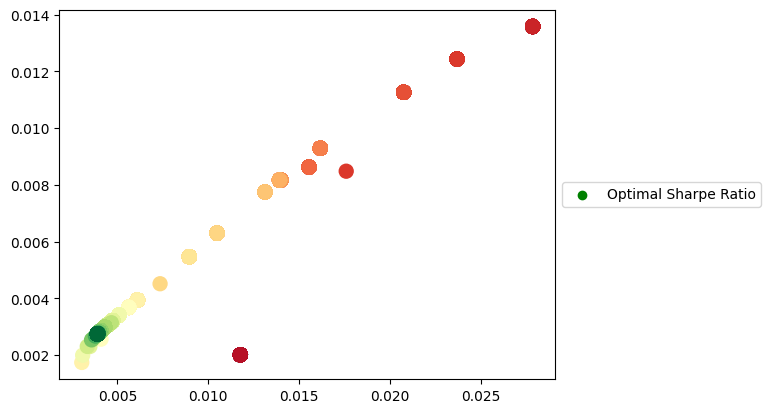
\includegraphics[width=0.5\textwidth]{./images/otimizacao_ibov.png}
                \par \footnotesize Fonte: próprio autor.
            \end{figure}

    \end{frame}
    \note{Convergência}
%-------------------------------------------------------





%-------------------------------------------------------
    \begin{frame}{Otimização com Parâmetros Reais}

        Comparação de modelos:

        \begin{itemize}
            \item Carteira ótima sem restrições reais;
            \item Carteira ótima com restrições reais e início aleatório;
            \item Carteira ótima com restrições reais e heurística.
        \end{itemize}
        
        Cenários: média e desvio padrão dos últimos 15, 30 e 60 dias nos componentes do Ibovespa. 

        Dados: conforme quadro \ref{quadro:coleta_dados} de coleta de dados.

        \begin{quadro}[H]
            \centering
            \caption{Parâmetros de mercado e investimento}
            \label{quadro:parametros}
            \begin{tabular}{ll}
                \hline
                \textbf{Parâmetro} & \textbf{Valor} \\
                \hline
                Capital de Investimento & R\$ 20.000,00 \\
                Valor Monetário Aceitável de Perda Diária & R\$ 100,00 \\
                Quantil da Distribuição Normal Padrão ao Nível de Confiança & 95\% \\
                Quantidade Inicial de Lotes do Ativo & 0 \\
                \hline
            \end{tabular}
            \par \footnotesize Fonte: próprio autor.
        \end{quadro}
        
    \end{frame}
    \note{Parâmetros e dados}
%-------------------------------------------------------





%-------------------------------------------------------
    \begin{frame}{Otimização com Parâmetros Reais}
        
        
        \begin{table}[htbp]
            \centering
            \caption{Resultados da otimização para os três cenários}
            \label{tab:resultados_opt}
            \resizebox{\columnwidth}{!}{%
            \begin{tabular}{clrrrr}
                \hline
                \textbf{Carteira} & \textbf{Método} & \textbf{Retorno} & \textbf{Risco} & \textbf{Sharpe do Otimizador} & \textbf{Tempo (s)} \\ \hline \hline
                15 & Sem Restrições & 15.80 & 16.14 & 0.9791 & 0.42 \\
                15 & Restrições e Aleatório & 3.96 & 39.83 & -0.0849 & 3.81 \\
                15 & Restrições com Heurística & 10.90 & 14.99 & 0.0751 & 3.70 \\
                30 & Sem Restrições & 43.98 & 61.49 & 0.7152 & 0.20 \\
                30 & Restrições e Aleatório & 23.37 & 121.18 & 0.1191 & 3.92 \\
                30 & Restrições com Heurística & 22.80 & 48.41 & 0.2321 & 3.88 \\
                60 & Sem Restrições & 64.01 & 106.91 & 0.5987 & 0.18 \\
                60 & Restrições e Aleatório & 1.15 & 48.36 & -0.1146 & 3.21 \\
                60 & Restrições com Heurística & 15.99 & 66.19 & -0.1700 & 10.13 \\
                \hline
            \end{tabular}%
            }
            \par \footnotesize Fonte: próprio autor.
        \end{table}

    \end{frame}
    \note{Resultados Cenários}
%-------------------------------------------------------





%-------------------------------------------------------
    \begin{frame}{Otimização com Parâmetros Reais}
        
        \begin{figure}[H]
            \centering
            \caption{Densidade de probabilidade das carteiras.}
            \label{fig:densidade_carteiras}
            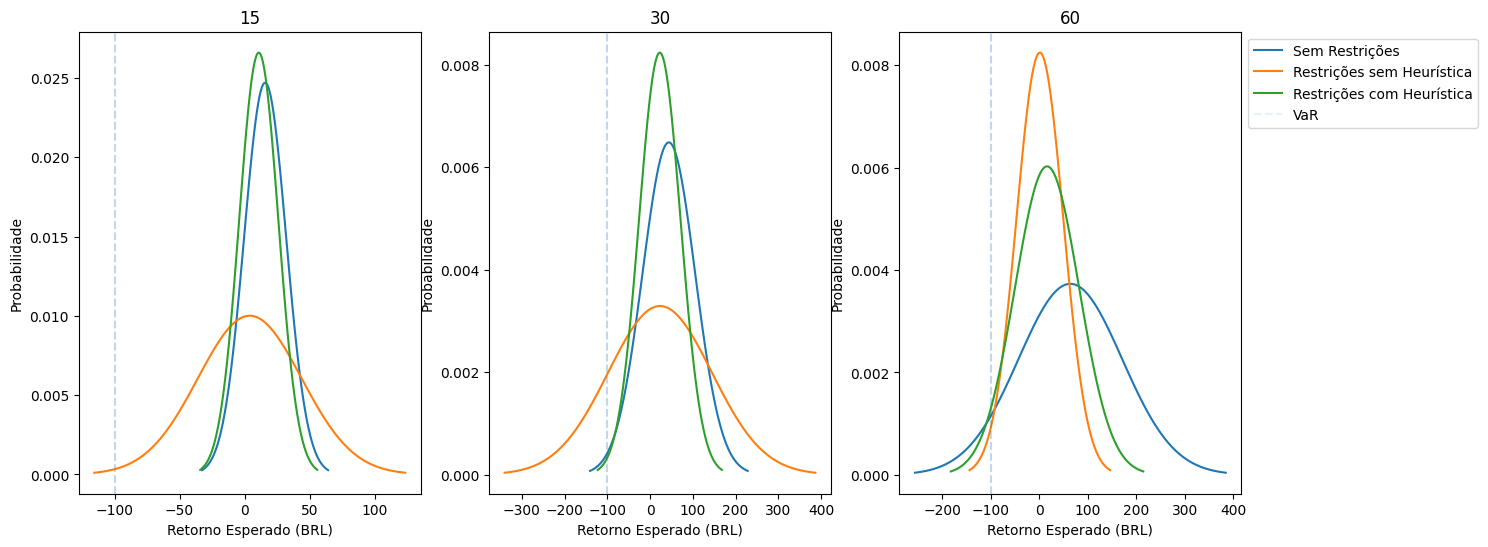
\includegraphics[width=\textwidth]{./images/distribuicao_carteiras.png}
            \par \footnotesize Fonte: próprio autor.
        \end{figure}

    \end{frame}
    \note{Curvas densidade}
%-------------------------------------------------------





%-------------------------------------------------------
    \begin{frame}{Otimização com Parâmetros Reais}
        
        \begin{table}[htbp]
            \centering
            \caption{Alocação da carteira de 30 dias}
            \label{tab:distribuicao_carteira_30}
            \begin{tabular}{rrr}
                \hline
                & Sem Restrições & Restrições com Heurística \\
                \hline\hline
               BRKM5 & 480 & - \\
               ENBR3 & 15620 & 18912 \\
               EQTL3 & 1400 & - \\
               GOLL4 & 80 & - \\
               IRBR3 & 820 & - \\
               JBSS3 & 520 & - \\
               PRIO3 & 540 & - \\
               RAIZ4 & 480 & - \\
               SLCE3 & 40 & - \\
               Livre de Risco & - & 1088 \\
               \hline
            \end{tabular}
            \par \footnotesize Fonte: próprio autor. 
        \end{table}

    \end{frame}
    \note{Alocação de ativos}
%-------------------------------------------------------





%-------------------------------------------------------
    \begin{frame}{Redes Neurais}
        
        \Large

        \begin{columns}
            \begin{column}{0.5\textwidth}

                Após a otimização das carteiras com atualização diária, é realizada a comparação dos retornos gerados pelas carteiras selecionadas no período de análise.

            \end{column}

            \begin{column}{0.5\textwidth}

                \begin{figure}[htbp]
                    \centering
                    \caption{Retornos gerados pelas carteiras.}
                    \label{fig:boxplot_inv}
                    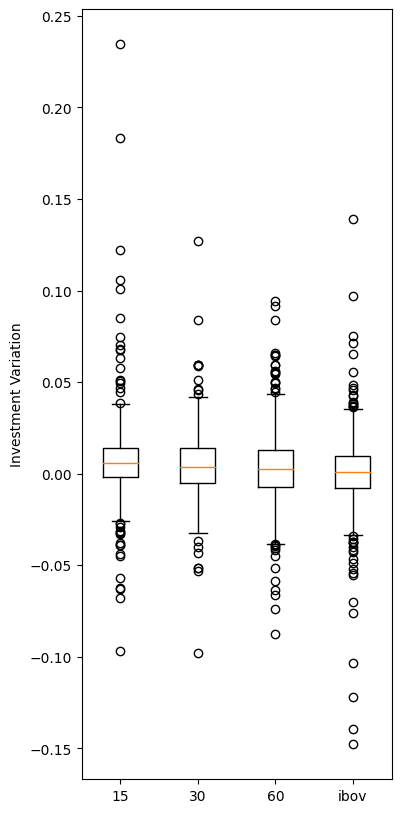
\includegraphics[width=0.4\textwidth]{./images/boxplot_inv.png}
                    \par \footnotesize Fonte: próprio autor.
                \end{figure}

            \end{column}
        \end{columns}

    \end{frame}
    \note{Análise de dados}
%-------------------------------------------------------





%-------------------------------------------------------
    \begin{frame}{Redes Neurais}
        
        \begin{columns}
            \begin{column}{0.5\textwidth}

                \begin{figure}[htbp]
                    \centering
                    \caption{Retorno acumulado das carteiras.}
                    \label{fig:retorno_acumulado}
                    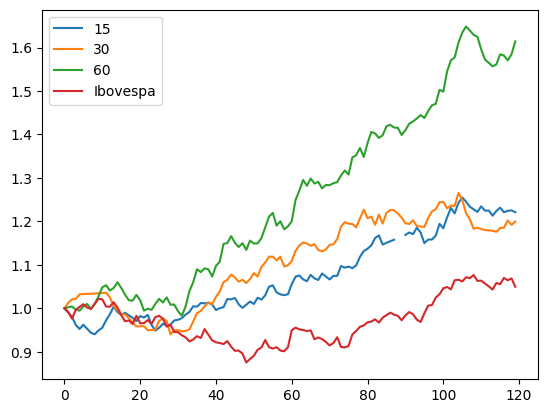
\includegraphics[width=0.9\textwidth]{./images/retorno_acumulado.png}
                    \par \footnotesize Fonte: próprio autor.
                \end{figure}

            \end{column}

            \begin{column}{0.5\textwidth}

                \begin{figure}[htbp]
                    \centering
                    \caption{Porcentagem de sucesso na otimização das carteiras.}
                    \label{fig:success_results}
                    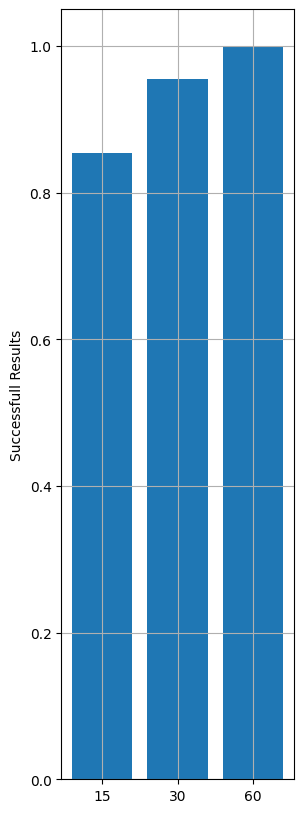
\includegraphics[width=0.3\textwidth]{./images/success_results.png}
                    \par \footnotesize Fonte: próprio autor.
                \end{figure}

            \end{column}
        \end{columns}

    \end{frame}
    \note{Análise de dados}
%-------------------------------------------------------




%-------------------------------------------------------
    \begin{frame}{Redes Neurais}


        \begin{columns}
            \begin{column}{0.5\textwidth}

                Estruturas: 
                \begin{itemize}
                    \item LSTM + Atenção de Bahdanau
                    \item LSTM + Auto Atenção
                    \item GRU + Atenção de Bahdanau
                    \item GRU + Auto Atenção
                \end{itemize}

            \end{column}

            \begin{column}{0.5\textwidth}


                \begin{figure}[htbp]
                    \centering
                    \caption{Acurácia para as redes avaliadas.}
                    \label{fig:accuracy}
                    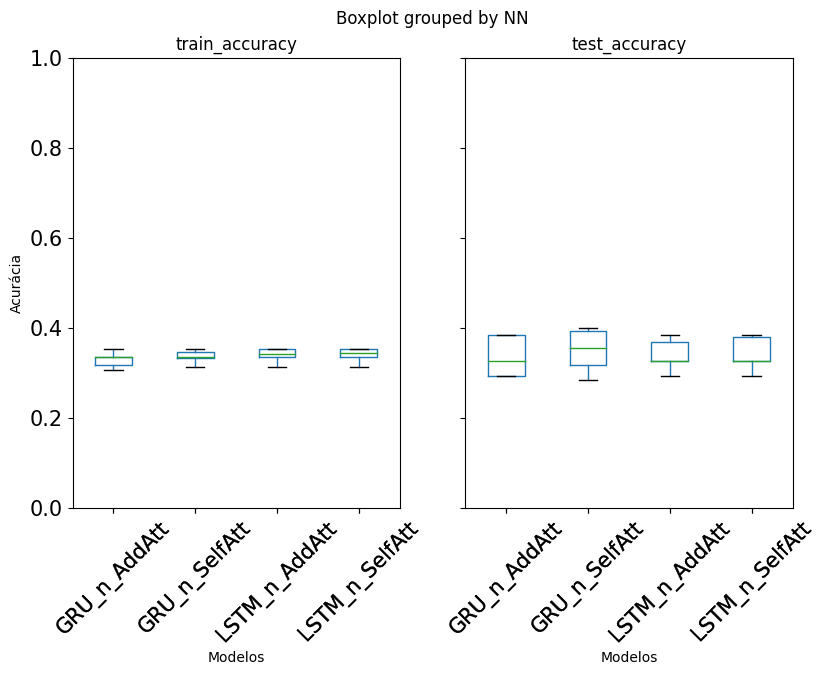
\includegraphics[width=0.98\textwidth]{./images/boxplot_val_01.png}
                    \par \footnotesize Fonte: próprio autor.
                \end{figure}

            \end{column}
        \end{columns}



    \end{frame}
    \note{Acurácia}
%-------------------------------------------------------





%-------------------------------------------------------
    \begin{frame}{Redes Neurais}

        \begin{columns}
            \begin{column}{0.5\textwidth}

                \begin{figure}[htbp]
                    \centering
                    \caption{Frequência dos atributos alvos do teste.}
                    \label{fig:freq}
                    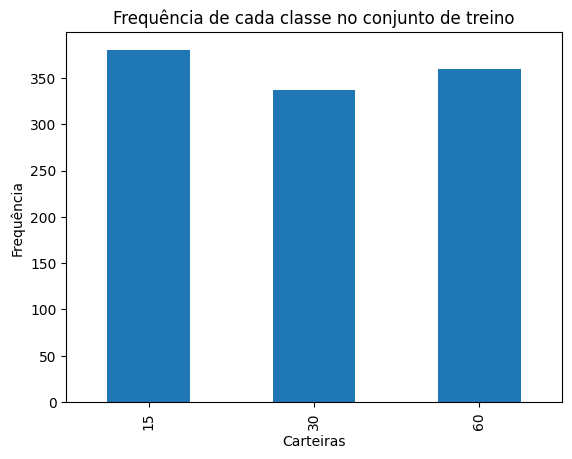
\includegraphics[width=0.98\textwidth]{./images/freq.png}
                    \par \footnotesize Fonte: próprio autor.
                \end{figure}

            \end{column}

            \begin{column}{0.5\textwidth}

                \begin{figure}[htbp]
                    \centering
                    \caption{Acurácia para as redes avaliadas, ampliado.}
                    \label{fig:boxplotval_zoom}
                    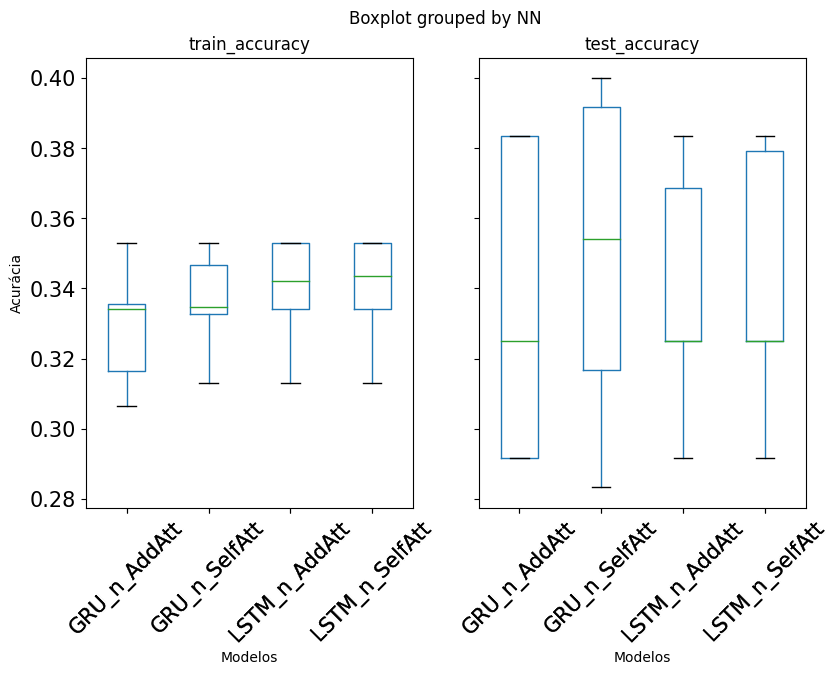
\includegraphics[width=0.98\textwidth]{./images/boxplotval_zoom.png}
                    \par \footnotesize Fonte: próprio autor.
                \end{figure}

            \end{column}
        \end{columns}


    \end{frame}
    \note{Acurácia}
%-------------------------------------------------------





%-------------------------------------------------------
    \begin{frame}{Redes Neurais}

        \begin{figure}[htbp]
            \centering
            \caption{Séries temporais de retorno acumulado geradas pelas predições das redes neurais.}
            \label{fig:backtest_ts}
            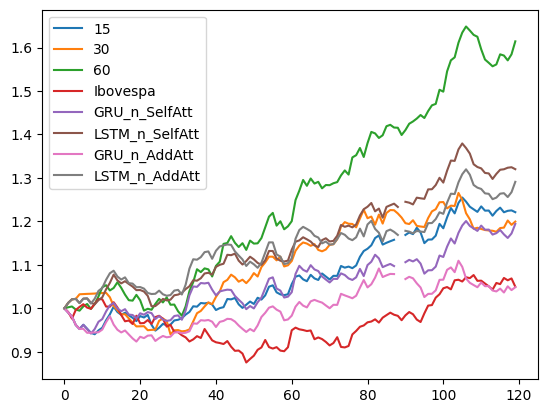
\includegraphics[width=0.5\textwidth]{./images/backtest_ts.png}
            \par \footnotesize Fonte: próprio autor.
        \end{figure}


    \end{frame}
    \note{Séries temporais}
%-------------------------------------------------------





%-------------------------------------------------------
    \begin{frame}{Redes Neurais}

        \begin{table}[htbp]
            \centering
            \caption{Índice Sharpe para as redes avaliadas e as carteiras.}
            \label{tab:sharpe}
            \begin{tabular}{rrrr}
                \hline
                & \textbf{Média} & \textbf{Desvio Padrão} & \textbf{Índice Sharpe} \\ \hline \hline
                GRU\_n\_SelfAtt & 0.0016 & 0.0119 & 0.13 \\
                LSTM\_n\_SelfAtt & 0.0024 & 0.0095 & 0.25 \\
                GRU\_n\_AddAtt & 0.0005 & 0.0105 & 0.04 \\
                LSTM\_n\_AddAtt & 0.0022 & 0.0114 & 0.19 \\
                15 & 0.0017 & 0.0101 & 0.17 \\
                30 & 0.0016 & 0.0108 & 0.15 \\
                60 & 0.0041 & 0.0131 & 0.31 \\
                \hline
                \par \footnotesize Fonte: próprio autor.
            \end{tabular}
        \end{table}

    \end{frame}
    \note{Tabela sharpe}
%-------------------------------------------------------